\chapter{Theoretical Foundation}
At its heart, this is a project about how meaning comes about in a world that

\section{Concepts in Context}
The language model presented here is based on the premise that conceptualisation happens in way that is fundamentally contextualised by an immediate situation in an environment.  The cognitive flexibility inherent in conceptualisations is reflected in the lexical ambiguity that is prevalent in language.  To the degree that it makes sense to talk about lexical semantics, the attribution of word meaning must be seen as a kind of \emph{a posterior} procedure, arising from the observation of how a word is generally related to a particular concept.

By the time a distributional model is generated from a large scale linguistic corpus, the blur from use to lexicalisation and then back towards figuration is already inherent in the statistical comportment of the data---so, for instance, it is not surprising to find that a word such as \emph{state} can be statistically associated, in terms of co-occurrence, with both words like \emph{solid}, in the conceptual sense of \textsc{physical state}, and words like \emph{Ohio}, in the sense of \textsc{American State}.

\begin{figure}[h]
    \centering
    \begin{subfigure}[h]{0.4\textwidth}
    \centering
	\caption{An Ambiguous Space}
	\label{fig:ambig}
	\begin{tikzpicture}[scale=0.06,baseline]
		\draw (0,0)--(-100,0)--(-100,-100)--(0,-100)--(0,0);

    	\draw (-52,-52) [above] node {state};
        \fill (-52,-52) circle[radius=1];

    	\draw (-55,-20) [above] node {solid};
        \fill (-55,-20) circle[radius=1];

    	\draw (-25,-48) [above] node {capital};
        \fill (-25,-48) circle[radius=1];

    	\draw (-48,-25) [below] node {liquid};
        \fill (-48,-25) circle[radius=1];
        
        \draw (-45,-75) [above] node {transform};
        \fill (-45,-75) circle[radius=1];
        
        \draw (-80,-55) [above] node {utah};
        \fill (-80,-55) circle[radius=1];
        
        \draw (-95,-45) [above] node {ohio};
        \fill (-95,-45) circle[radius=1];

        \node at (-50,-102.5) [single arrow,draw,rotate=90,minimum height=40,minimum width=40,inner sep=15,opacity=0] {};
        
    \end{tikzpicture}
	\end{subfigure}
	\hspace{15pt}
	\begin{subfigure}[h]{0.4\textwidth}
	\centering
	\caption{A Refined Space}
	\label{fig:refine}
	\begin{tikzpicture}[scale=0.06,baseline]
    	\draw (0,0)--(-100,0)--(-100,-100)--(-57.5,-100);
        \draw (-42.5,-100)--(0,-100)--(0,-57.5);
        \draw (0,-42.5)--(0,0);

    	\draw (-52,-52) [above] node {state};
        \fill (-52,-52) circle[radius=1];
        \draw[dashed,->] (-52,-52)--(-52,-100);
        \draw (-52,-100) node {x};
        \draw[dashed,->] (-52,-52)--(0,-52);
        \draw (0,-52) node [rotate=90] {x};

    	\draw (-55,-20) [above] node {solid};
        \fill (-55,-20) circle[radius=1];
        \draw[dashed,->] (-55,-20)--(-55,-100);
        \draw (-55,-100) node {x};
        \draw[dashed,->] (-55,-20)--(0,-20);
        \draw (0,-20) node [rotate=90] {x};

    	\draw (-25,-48) [above] node {capital};
        \fill (-25,-48) circle[radius=1];
        \draw[dashed,->] (-25,-48)--(-25,-100);
        \draw (-25,-100) node {x};
        \draw[dashed,->] (-25,-48)--(0,-48);
        \draw (0,-48) node [rotate=90] {x};

    	\draw (-48,-25) [below] node {liquid};
        \fill (-48,-25) circle[radius=1];
        \draw[dashed,->] (-48,-25)--(-48,-100);
        \draw (-48,-100) node {x};
        \draw[dashed,->] (-48,-25)--(0,-25);
        \draw (0,-25) node [rotate=90] {x};
        
        \draw (-45,-75) [above] node {transform};
        \fill (-45,-75) circle[radius=1];
        \draw [dashed,->] (-45,-75)--(-45,-100);
        \draw (-45,-100) node {x};
        \draw [dashed,->] (-45,-75)--(0,-75);
        \draw (0,-75) node [rotate=90] {x};
        
        \draw (-80,-55) [above] node {utah};
        \fill (-80,-55) circle[radius=1];
        \draw [dashed,->] (-80,-55)--(-80,-100);
        \draw (-80,-100) node {x};
        \draw [dashed,->] (-80,-55)--(0,-55);
        \draw (0,-55) node [rotate=90] {x};
        
        \draw (-95,-45) [above] node {ohio};
        \fill (-95,-45) circle[radius=1];
        \draw [dashed,->] (-95,-45)--(-95,-100);
        \draw (-95,-100) node {x};
        \draw [dashed,->] (-95,-45)--(0,-45);
        \draw (0,-45) node [rotate=90] {x};
        
        \node at (3,-50) {\Huge\}};
        \node at (-50,-103) [rotate=-90] {\Huge\}};
%        \node at (-50,-103) [rotate=-90] {\fontsize{80pt}{4em}\selectfont \}};
        
        \node at (-50,-102.5) [single arrow,draw,rotate=90,minimum height=40,minimum width=40,inner sep=15] {};
        \node at (-50,-107) {\textsc{physical}};
        \node at (2.5,-50) [single arrow,draw,rotate=180,,minimum height=40,minimum width=40,inner sep=15] {};
        \node at (7,-50) [rotate=90] {\textsc{american}};
    \end{tikzpicture}
    \end{subfigure}
    \caption{An ambiguous two-dimensional space of words relating to the term \emph{cat} (a), and a refined space where, based on two different one-dimensional projections, two different conceptual mappings of \emph{cat} emerge as word clusters (b).}
\end{figure}

\section{A Literal, Dynamic Language Model}

The model described here is characterised by two crucial features:

\begin{enumerate}
\item The dimensional features of the space are literally interpretable, in that they correspond to information theoretical statistics about the co-occurrence of words in a large scale corpus.
\item Following on this first point, the model operates by a procedure of continuously unfolding projections of subspaces, with the character of these projections determined by a continuous dimensional analysis based on input terms.
\end{enumerate}

In the first instance, the maintenance of dimensions populated by statistics pulled directly from a corpus traversal differentiates this approach from recent work by the likes of \cite{MikolovEA2013b} and \cite{PenningtonEA2014}, who have made use of neural networks and matrix factorisation to build models which perform well on hand-crafted test sets designed to test the models' performance on specific aspects of conceptualisation.  It is precisely the statistically concrete nature of the present model which allows it to remain conceptually dynamic.  Because the model's dimensions correspond literally to co-occurrence terms, an analysis of the dimensions that contribute strongly to terms observed as occurring in a particular contextual context can be drawn out and used to project a subspace from a base model.

\section{The Geometry of Metaphor}
The contextual dynamism of concepts is implicit in the isomorphic mappings between conceptual schemes at the root of \citepos{Lakoff} conceptual metaphors.  It is the internal anatomy of each conceptual scheme, produced by the environmental and consequent cultural entanglements inherent in language, that allows the alignment of conceptual schemes: there is always an implicit geometric foundation to these mappings (and this foundation is often rather more explicit, as in the case of, for example, orientation and conduit metaphors).  This project seeks to realise a practical implementation of this theoretical stance, in particular by utilising the geometric qualities of the contextualised subspaces that have already been described.  In particular, the al

There is once again a point of comparison with the models that have been described in the contemporary NLP literature here.  The analogy completions performed by the model of, for instance, \cite{MikolovEA2013b} employ a clever layer of basic linear algebra to word-vectors derived through the complex non-linear processing of corpus data.  These operations are, however, dependent on a certain consistency of scale within a space.  The algebraic relationship $\overrightarrow{king}-\overrightarrow{queen} = \overrightarrow{man}-\overrightarrow{woman}$, for instance, which has been discussed extensively in recent papers, depends on a comparability not only in terms of orientation but also in terms of distance between the spaces of \textsc{royals} and \textsc{people}.  This is a special category of analogy within a distributional model, however, as there are demonstrably comparable conceptualisations mappable from word clusterings of various scales.

By instead relying on the general geometric property of congruity rather than the specific scale of a space, the model described here offers a more robust approach to drawing connections between spaces.  If a concept is represented as a cluster of words that emerge in a distributional semantic subspace, then the theory here is that there should be mappings between the words in two different such subspaces which, taken as a whole, substantiate a conceptual metaphor.  The intuition here can be related to a more traditional transference view of metaphor: there will be some notable overlap between the co-occurrence profiles of the respective distributional spaces of, for instance, \textsc{surgery} and \textsc{butchery}.  By identifying this overlap, it should be possible to draw out correspondences between conceptual components such as \emph{scalpel} and \emph{cleaver}, and this in turn allows for the postulation of an alignment between the spaces which represents a metaphor.  Thus it is the geometry of the spaces which ultimately affords the opportunity for constructing a new semantic connection between conceptual domains, and the evident transference of intensions might be interpreted as an \emph{a posteriori} logical artefact of this process.

\begin{figure}
	\centering
	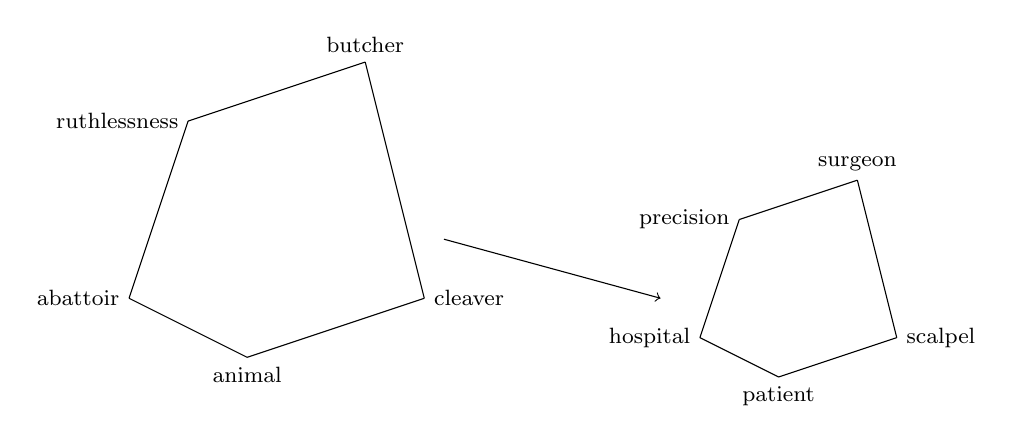
\begin{tikzpicture}[scale=0.25]
		\draw (6,15)--(15,18) node [above] {\footnotesize butcher};
		\draw (15,18)--(18,6) node [right] {\footnotesize cleaver};
		\draw (18,6)--(9,3) node [below] {\footnotesize animal};
		\draw (9,3)--(3,6)node [left] {\footnotesize abattoir};
		\draw (3,6)--(6,15) node [left] {\footnotesize ruthlessness};
		
		\draw [->] (19,9)--(30,6);
		
		\draw (34,10)--(40,12) node [above] {\footnotesize surgeon};
		\draw (40,12)--(42,4) node [right] {\footnotesize scalpel};
		\draw (42,4)--(36,2) node [below] {\footnotesize patient};
		\draw (36,2)--(32,4) node [left] {\footnotesize hospital};
		\draw (32,4)--(34,10) node [left] {\footnotesize precision};
	\end{tikzpicture}
	\caption{Congruences discovered in subregions of a vector space model suggest metaphoric mappings.  The regions do not necessarily have to be of the same scale in order to identify a possible alignment.}
\end{figure}
